\subsection{BlissBook}
\begin{figure}[h]
	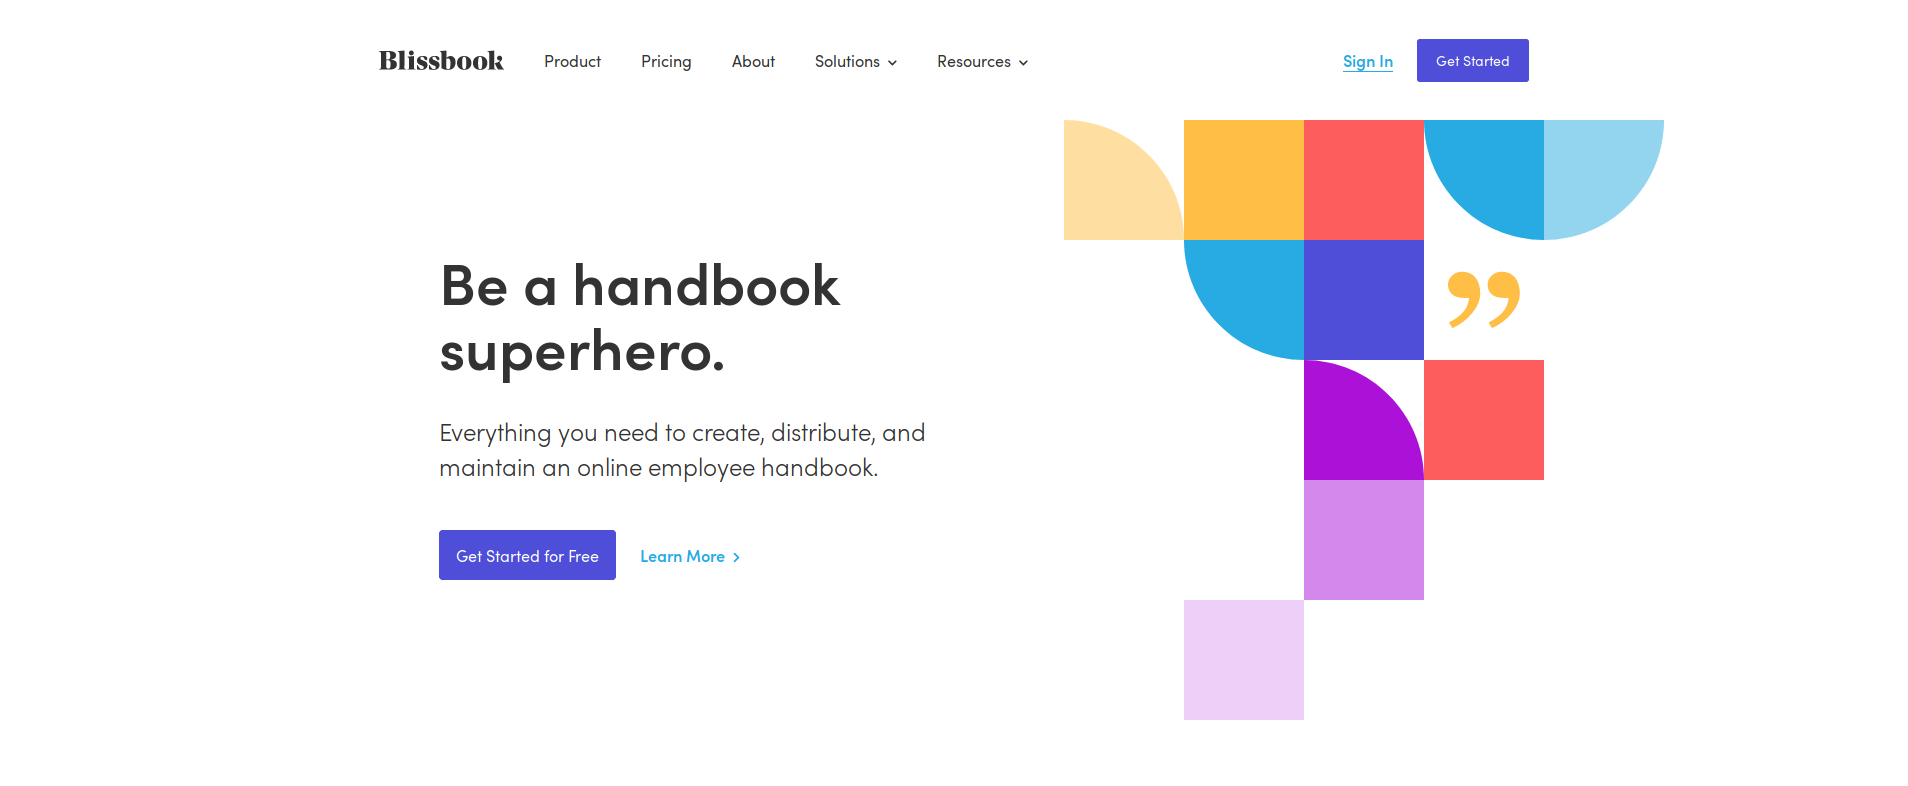
\includegraphics[width=1\textwidth]{billeder/BlissBooks.png}
	\caption{BlissBook landing page}
\end{figure}
<<<<<<< HEAD
<<<<<<< HEAD
% husk at referere til figuren i teksten
BlissBook is a \textit{Software as a Service} (SaaS) employee handbook system, developed by the company of the same name starting in 2013. % cite https://blissbook.com/about
This chapter is mostly based upon information from their website (\url{https://blissbook.com})
=======
BlissBook is a \textit{Software as a Service} (SaaS) employee handbook system, developed by the company of the same name started in 2013. % cite https://blissbook.com/about
This chapter is mostly based upon information from their website (\url{https://blissbook.com}).
>>>>>>> e74c51816e3cb9cb21d9ffd80a713ca3ec7d8353
=======
BlissBook is a \textit{Software as a Service} (SaaS) employee handbook system, developed by the company of the same name started in 2013. % cite https://blissbook.com/about
This chapter is mostly based upon information from their website (\url{https://blissbook.com}).
>>>>>>> e74c51816e3cb9cb21d9ffd80a713ca3ec7d8353


BlissBook is based on a rich text editor which supports collabrative editing, and has features such as access control, digital signatures to keep track of which employees have read which handbooks, and sending notifications to employees when new versions are released.

<<<<<<< HEAD
<<<<<<< HEAD
As they are a SaaS platform, all the content and software is actually hosted on their servers. In SU, this would be a local presentation client-server pattern.
% SU? hvis det er system development er det noget man burde nævne her? 
On their server, they guarantee a 99.9\% uptime, and exports of all data on the platform, even after a canceled subscription. How long they keep the data is not specified.

On the security front, the BlissBook website does not mention any certificatations on their software, besides them offering AES-256 encryption. % https://blissbook.com/information-security
They do not freely offer up any sort of self-hosting solution, which security-conscious corporations may be very interested in. But as our contact does not have any specific security concern besides data integrity, the SaaS structure is in the end of an advantage.
% vi skal nok blive enige om hvad vi kalder Pia i rapporten
=======
As they are a SaaS platform, all the content and software is hosted on their servers. In SU, this would be a local presentation client-server pattern.
On their server, they guarantee a 99.9\% uptime, and exports of all data on the platform, even after a canceled subscription. How long they keep the data is not specified.

On the security front, the BlissBook website does not mention any certificatations on their software, besides them offering AES-256 encryption. % https://blissbook.com/information-security
They do not freely offer up any sort of self-hosting solution, which security-conscious corporations may be very interested in. But as our contact does not have any specific security concerns besides data integrity, the SaaS structure is in the end of an advantage.
>>>>>>> e74c51816e3cb9cb21d9ffd80a713ca3ec7d8353
=======
As they are a SaaS platform, all the content and software is hosted on their servers. In SU, this would be a local presentation client-server pattern.
On their server, they guarantee a 99.9\% uptime, and exports of all data on the platform, even after a canceled subscription. How long they keep the data is not specified.

On the security front, the BlissBook website does not mention any certificatations on their software, besides them offering AES-256 encryption. % https://blissbook.com/information-security
They do not freely offer up any sort of self-hosting solution, which security-conscious corporations may be very interested in. But as our contact does not have any specific security concerns besides data integrity, the SaaS structure is in the end of an advantage.
>>>>>>> e74c51816e3cb9cb21d9ffd80a713ca3ec7d8353

One of the greatest disadvantages to this system is that all the files in the system need to be written in BlissBook's own online editor. This would present a great difficulty, as all existing documentation which our contact relies on is written mostly in word documents, but also spreadsheets, pictures, and others.
% det ved word document ligger det ikke senere i rapporten i bruger analyse? 

Additionally, the solution does not seem to be fitted to the use case of standards compliance, but rather handbooks for human resources use cases. While they do have a system for external handbook consultants, they are again focusing on HR consultants. (\url{https://blissbook.com/employee-handbook-management})
